\section{Theoretical Analysis}
\label{sec:analysis}

\subsection{Exercise 1} \label{sec:Ex1Theo}

In this exercise, the circuit shown in Figure~\ref{fig:CircuitDraw} is analysed theoretically for $t<0$, by using the node method. The Kirchhoff Current Law (KCL) states that the sum of the currents converging or diverging in a node is null. Using KCL and Ohm's Law (which can also be written as $I=VG$) in nodes not connected to voltage sources and additional equations for nodes related by voltage sources, it is possible to obtain a linear system from which the node voltages $V_1$ to $V_8$ are obtained. Using these values and Ohm's Law, the currents in all branches can be determined.

\par
It is worth mentioning that the current passing through the capacitor is given by $i_c=C\frac{dv_c}{dt}$. However, it is assumed that the voltages in the capacitor's terminals have already achieved static values  a long time ago, thus $i_c=0$. 

\par
\vspace{1mm}

The following linear system is obtained:

\begin{equation}
  \begin{pmatrix}
    1 & 0 & 0 & 0 & 0 & 0 & 0 & 0 \\
    -\frac{1}{R_1} & \frac{1}{R_1}+\frac{1}{R_2}+\frac{1}{R_3} & -\frac{1}{R_2} & 0 & -\frac{1}{R_3} & 0 & 0 & 0 \\
    0 & -K_b-\frac{1}{R_2} & \frac{1}{R_2} & 0 & K_b & 0 & 0 & 0 \\
    0 & 0 & 0 & 1 & 0 & 0 & 0 & 0 \\
    0 & -\frac{1}{R_3} & 0 & 0 & \frac{1}{R_3}+\frac{1}{R_4}+\frac{1}{R_5} & -\frac{1}{R_5} & -\frac{1}{R_7} & \frac{1}{R_7} \\
    0 & K_b & 0 & 0 & -\frac{1}{R_5}-K_b & \frac{1}{R_5} & 0 & 0 \\
    0 & 0 & 0 & 0 & 0 & 0 & \frac{1}{R_6}+\frac{1}{R_7} & -\frac{1}{R_7} \\
    0 & 0 & 0 & 0 & 1 & 0 & \frac{K_d}{R_6} & -1
  \end{pmatrix}
  \begin{pmatrix}
    V_1  \\
    V_2  \\
    V_3  \\
    V_4  \\
    V_5  \\
    V_6  \\
    V_7  \\
    V_8  \\
  \end{pmatrix}
  =
  \begin{pmatrix}
    V_s \\
    0   \\
    0   \\
    0   \\
    0   \\
    0   \\
    0   \\
    0   \\
  \end{pmatrix}
  \label{eq:Exercise1LinearSystem}
\end{equation}

The matrix shown above isn't symmetrical because of the presence of dependent sources in this circuit. The values obtained by solving the linear system above, using Octave, are shown in Table \ref{tab:Exercise1Theoretical}.

\begin{table}[H]
  \centering
  \begin{tabular}{|c|c|}
    \hline
        {\bf Designation} & {\bf Value [A or V]} \\ \hline
        \input{Exercise1.tex}
  \end{tabular}
  \caption{Values of node voltages (in volts) and currents (in amperes). Current $I_i$ corresponds to the current passing through resistance $R_i$. Node 4 is connected to GND, thus it isn't necessary to show its voltage value ($V_4=0$) above.} 
  \label{tab:Exercise1Theoretical}
\end{table}


\subsection{Exercise 2} \label{sec:Ex2Theo}

In this exercise, the goal is to obtain $R_{eq}$, the value of the equivalent resistance as seen from the capacitor's terminals. According to Thévenin's Theorem, it is possible to replace the linear sub-circuit connected to the capacitor's terminals by a voltage source connected with the resistor. In order to calculate $R_{eq}$ by Thévenin's Theorem, we must have $V_s=0$ (all independent sources of the sub-circuit connected to the capacitor's terminals must be switched off). By replacing the capacitor with a voltage source $V_x=V_6-V_8$, where $V_6$ and $V_8$ are the voltages determined in Section \ref{sec:Ex1Theo}, the current $I_x$ supplied by $V_x$ can be calculated by applying the node method to this new circuit - using Ohm's Law, the equivalent resistance is computed as $R_x=\frac{V_x}{I_x}$. The linear system and the node voltages and branch currents in this case are the following:

\begin{equation}
  \begin{pmatrix}
    1 & 0 & 0 & -1 & 0 & 0 & 0 & 0 \\
    -\frac{1}{R_1} & \frac{1}{R_1}+\frac{1}{R_2}+\frac{1}{R_3} & -\frac{1}{R_2} & 0 & -\frac{1}{R_3} & 0 & 0 & 0 \\
    0 & -K_b-\frac{1}{R_2} & \frac{1}{R_2} & 0 & K_b & 0 & 0 & 0 \\
    0 & 0 & 0 & 1 & 0 & 0 & 0 & 0 \\
    0 & K_b-\frac{1}{R_3} & 0 & 0 & \frac{1}{R_3}+\frac{1}{R_4}-K_b & 0 & -\frac{1}{R_7} & \frac{1}{R_7} \\
    0 & 0 & 0 & 0 & 0 & 1 & 0 & -1 \\
    0 & 0 & 0 & 0 & 0 & 0 & \frac{1}{R_6}+\frac{1}{R_7} & \frac{1}{R_7} \\
    0 & 0 & 0 & 0 & 1 & 0 & -\frac{K_d}{R_6} & -1 \\
  \end{pmatrix}
  \begin{pmatrix}
    V_1  \\
    V_2  \\
    V_3  \\
    V_4  \\
    V_5  \\
    V_6  \\
    V_7  \\
    V_8  \\
  \end{pmatrix}
  =
  \begin{pmatrix}
    0 \\
    0 \\
    0 \\
    0 \\
    0 \\
    V_x \\
    0 \\
    0 \\
  \end{pmatrix}
  \label{eq:Exercise2LinearSystem}
\end{equation}

\begin{table}[H]
  \centering
  \begin{tabular}{|c|c|}
    \hline
        {\bf Designation} & {\bf Value [A or V]} \\ \hline
        $I_1$ & 1.181855E-03 \\ \hline 
$I_2$ & 1.237205E-03 \\ \hline 
$I_3$ & 5.535009E-05 \\ \hline 
$I_4$ & -2.553371E-04 \\ \hline 
$I_5$ & -1.048370E-03 \\ \hline 
$I_6$ & -1.437192E-03 \\ \hline 
$I_7$ & -1.437192E-03 \\ \hline 
$I_b$ & 1.237205E-03 \\ \hline 
$I_c$ & -2.285575E-03 \\ \hline 
$I_{V_s}$ & 1.181855E-03 \\ \hline 
$I_{V_d}$ & 8.483826E-04 \\ \hline 
$V_1$ & 0.000000E+00 \\ \hline 
$V_2$ & 1.229766E+00 \\ \hline 
$V_3$ & 3.706477E+00 \\ \hline 
$V_5$ & 1.060067E+00 \\ \hline 
$V_6$ & 4.240919E+00 \\ \hline 
$V_7$ & -2.955652E+00 \\ \hline 
$V_8$ & -4.401288E+00 \\ \hline 

  \end{tabular}
  \caption{Values of node voltages (in volts) and branch currents (in amperes). Current $I_i$ corresponds to the current passing through resistance $R_i$.}
  \label{tab:Exercise2Theoretical}
\end{table}

Now, the current going through the equivalent resistor can be calculated as $I_x=I_b-I_5=-I_{V_x}$ (KCL in node 6). It must be stated that the current going through $R_{eq}$ (i.e., from + to - in $R_{eq}$) is flowing in the oposite direction of the current ``passing through'' voltage source $V_x$, i.e., the current going from + to - in $V_x$, thus the equation shown before.
\par
Finally, one can compute the time constant as $\tau=R_xC$. The final results are shown in Table \ref{tab:Exercise2_1Theoretical}.

\begin{table}[H]
  \centering
  \begin{tabular}{|c|c|}
    \hline
        {\bf Designation} & {\bf Value [A or V or $\Omega$ or s]} \\ \hline
        \input{Exercise2_1.tex}
  \end{tabular}
  \caption{Values determined for $V_x$ [V], $I_x$ [A], $R_{eq}$ [$\Omega$] and $\tau$ [s].}
  \label{tab:Exercise2_1Theoretical}
\end{table}

This procedure must be done in order to determine $R_{eq}$, which is used to obtain the time constant. This static analysis also allows us to obtain the initial condition $v_6(0)$, which will also be used to compute the natural and final solutions, because we may consider that, for $t=0$, $v_s=0$ and $V_6-V_8=V_x$. It is worth noting that, according to the expression for $v_s(t)$ given in Figure \ref{fig:CircuitDraw}, $v_s(0)=V_s$, so the change in value for $v_s$ would occur instantaneously afterwards, in an instant $t=\delta$; however, it is valid to consider it to be happening at $t=0$, because it doesn't change the overall solution.

\subsection{Exercise 3} \label{sec:Ex3Theo}

Using the results from the previous exercise, we can infer that the circuit shown in Figure \ref{fig:CircuitDraw} can be simplified into a circuit with the independent voltage source, a resistance $R_{eq}$ and the capacitor. We also have that $v_{6n}(+\infty)=0$, because, as seen in Table \ref{tab:Exercise2Theoretical}, $v_8=0$, and it will continue to be that way, and the capacitor will eventually completely discharge. Thus, the general form for the wanted natural solution, as learnt in class, is given by

\begin{equation} \label{eq:NaturalSolution}
  v_{6n}(t)=v_{6n}(+\infty)+[v_{6n}(0)-v_{6n}(+\infty)] e^{-\frac{t}{RC}}=v_{6n}(0) e^{-\frac{t}{RC}}
\end{equation}

Where $t$ stands for time and $R$ for the (equivalent) resistance. The graph shown below is obtained by plotting Eq. \ref{eq:NaturalSolution} in Octave.

\begin{figure}[H]
  \centering
  \includegraphics[width=0.8\linewidth]{natural.eps}
  \caption{Natural solution $v_{6n}(t)$ in the time interval [0,20] ms.}
  \label{fig:NaturalSolutionGraph}
\end{figure}


\subsection{Exercise 4} \label{sec:Ex4Theo}

In this exercise, the forced solution for the voltage in node 6, $v_{6f}(t)$, will be determined for the time interval [0,20] ms. Because we are dealing with a forced solution with sinusoidal excitation, given by $v_s(t)=sin(2\pi ft)$, with $f=1$kHz, it becomes much more efficient to use phasors. As suggested, a phasor voltage source $V_s=1$ will be used. The correspondant phase is $\phi_{V_s}=0$; therefore, in this forced solution analysis, the voltages will be considered as given by $sin$ functions, as opposed to $cos$ functions, as was learnt in class. This won't change the overall results, but will be important to take into account when analysing the phases plotted in Sections \ref{sec:Ex6Theo} and \ref{sec:Ex5Sim}. In addition to this, $C$ is replaced by its impedance, $Z_C$. This impedance is given by $Z_C=\frac{1}{j\omega C}$, with $j$ being the imaginary unit and $\omega=2\pi f$.
\par
By running nodal analysis as in the previous sections, the following linear system is obtained:
\vspace{-2mm}
\begin{equation}
  \begin{pmatrix}
    1 & 0 & 0 & 0 & 0 & 0 & 0 & 0 \\
    -\frac{1}{R_1} & \frac{1}{R_1}+\frac{1}{R_2}+\frac{1}{R_3} & -\frac{1}{R_2} & 0 & -\frac{1}{R_3} & 0 & 0 & 0 \\
    0 & -K_b-\frac{1}{R_2} & \frac{1}{R_2} & 0 & K_b & 0 & 0 & 0 \\
    0 & 0 & 0 & 1 & 0 & 0 & 0 & 0 \\
    0 & -\frac{1}{R_3} & 0 & 0 & \frac{1}{R_3}+\frac{1}{R_4}+\frac{1}{R_5}  & -\frac{1}{R_5}-jwC & -\frac{1}{R_7} & \frac{1}{R_7}+jwC \\
    0 & K_b & 0 & 0 & -K_b-\frac{1}{R_5} & \frac{1}{R_5}+jwC & 0 & -jwC \\
    0 & 0 & 0 & 0 & 0 & 0 & \frac{1}{R_6}+\frac{1}{R_7} & -\frac{1}{R_7} \\
    0 & 0 & 0 & 0 & 1 & 0 & \frac{K_d}{R_6} & -1 \\
  \end{pmatrix}
  \begin{pmatrix}
    V_1  \\
    V_2  \\
    V_3  \\
    V_4  \\
    V_5  \\
    V_6  \\
    V_7  \\
    V_8  \\
  \end{pmatrix}
  =
  \begin{pmatrix}
    Vs  \\
    0   \\
    0   \\
    0   \\
    0   \\
    0  \\
    0   \\
    0   \\
  \end{pmatrix}
  \label{eq:Exercise4LinearSystem}
\end{equation}

The complex amplitudes (phasors) in the nodes, obtained by solving the linear system above, are shown below.
\vspace{-3mm}
\begin{table}[H]
  \centering
  \begin{tabular}{|c|c|}
    \hline
        {\bf Designation} & {\bf Value [V]} \\ \hline
        \input{Exercise4.tex}
  \end{tabular}
  \caption{Complex values of the phasors in the nodes (in volts).}
  \label{tab:Exercise4Theoretical}
\end{table}

Having the value of the phasor $V_6$, the respective sine function is easily obtained with Octave. It has the same frequency as the voltage source's and its phase and amplitude are given by the phasor shown in Table \ref{tab:Exercise4Theoretical}. The sinusoidal forced solution is plotted in Figure \ref{fig:ForcedSolutionGraph}.

\begin{figure}[H]
  \centering
  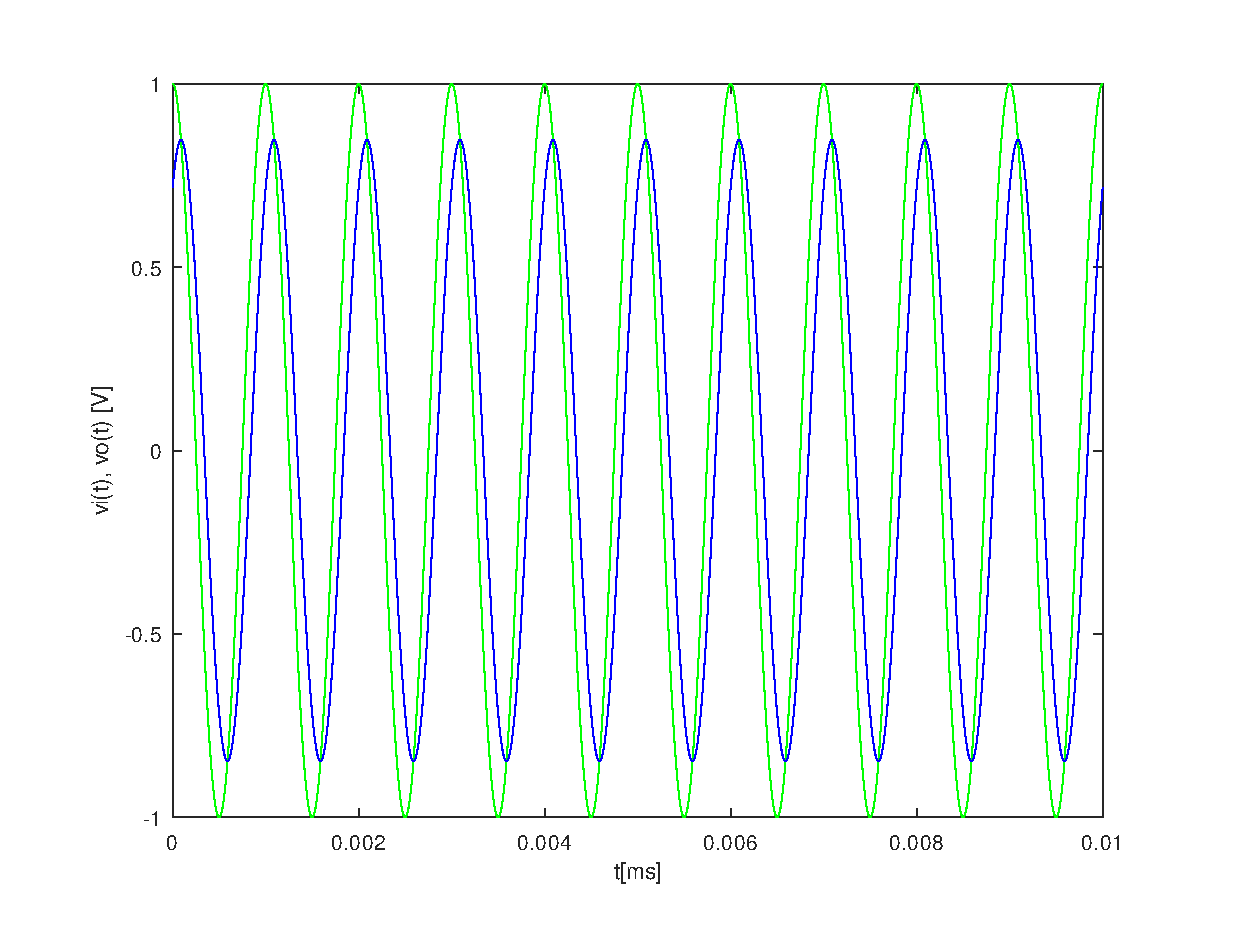
\includegraphics[width=0.65\linewidth]{forced.eps}
  \caption{Forced solution $v_{6f}(t)$ in the time interval [0,20] ms. To be noted that $V_6$ written above refers to the absolute value of the phasor, not the phasor itself. The phase $\phi$ is the symmetric of the phasor's argument.}
  \label{fig:ForcedSolutionGraph}
\end{figure}

\subsection{Exercise 5} \label{sec:Ex5Theo}

In Figure \ref{fig:final}, the final solution for $v_6 (t)$ is plotted alongside $v_s(t)$, which is given by the branch function presented in Figure \ref{fig:CircuitDraw}. The value of $v_6(t)$ is given by $v_{6n}(t)+v_{6f}(t)$ for $t>0$ (obtained by superimposing the natural and forced solutions, previously determined), by the value obtained in Section \ref{sec:Ex1Theo} for $t<0$ and by the value obtained in Section \ref{sec:Ex2Theo} for $t=0$.


\begin{figure}[H] \centering
  \includegraphics[width=0.8\linewidth]{final.eps}
  \caption{Final solution $v_6(t)$ and $v_s(t)$ in time interval [-5, 20] ms.}
  \label{fig:final}
\end{figure}

We can notice that neither $v_6$ nor $v_s$ are continuous functions. What must be continuous is $v_c$, the voltage drop in the capacitor's terminals; the voltages in the nodes may have discontinuities in order to make sure this stays true. A capacitor cannot be discharged instantaneously: it does it through its equivalent resistor according to the time constant $\tau$.


\subsection{Exercise 6} \label{sec:Ex6Theo}

Finally, the magnitudes and the phases of the frequency responses $v_c(f)=v_6(f)-v_8(f)$, $v_6(f)$ and $v_s(f)$ will be plotted for the frequency range 0.1 Hz to 1 MHz. The magnitude and phase of $v_c(f)$ are easily inferred by its respective branch function, given in Figure \ref{fig:CircuitDraw}. In its turn, using Octave and the linear system given in Section \ref{sec:Ex4Theo}, it was possible to get expressions for $v_6$ and $v_8$ in terms of frequency, from which the wanted plots were obtained.

\begin{figure}[H]
  \footnotesize
  \begin{subfigure}{0.5\linewidth}
    \footnotesize
    \centering
    % include first image
    \includegraphics[width=1.05\linewidth]{dBoct.eps}
    \footnotesize
    \caption{Magnitudes of $v_s(f)$, $v_6(f)$ and $v_c(f)$.}
    \label{fig:final_magnitude}
  \end{subfigure}
  \begin{subfigure}{0.5\linewidth}
    \centering
    % include second image
    \includegraphics[width=1.05\linewidth]{phaseoct.eps}  
    \caption{Phases of $v_s(f)$, $v_6(f)$ and $v_c(f)$.}
    \label{fig:final_phase}
  \end{subfigure}
\end{figure}


The results obtained in Figures (\ref{fig:final_magnitude}) and (\ref{fig:final_phase}) seem to behave as predicted. The magnitude and phase of $v_s$ are constant, as they are given by the sine function shown in Figure \ref{fig:CircuitDraw}. Again, it is worth mentioning that we are considering the phases of $sin$ functions, not $cos$ functions - this does not change the overall solutions, but it does shift the phases by -$\frac{\pi}{2}$. The impedance of the capacitor, given by $Z_c=\frac{1}{j\omega C}$, with $\omega=2\pi f$, decreases as the frequency increases. Therefore, the magnitude of the voltage in the capacitor will tend to zero - because the graph is plotted in dB, it tends to $-\infty$. In fact, this magnitude is given by $V_c=\frac{V_s}{\sqrt{1+\omega^{2}R^{2}C^{2}}}$, thus its decrease. We can also see that the magnitude of $V_6$ tends to change to a particular value as the frequency increases; we know that this must be happening in a way that makes it so that the magnitude of $V_6-V_8(=V_c)$ tends to zero.
\par
As for the phase of $v_c$, we can see that it tends to $-\frac{\pi}{2}$ rad $=$ $-90^{o}$ as the frequency increases. This was to be expected, because the phase delay of the voltage in the capacitor is given by $\phi_{v_{c}}=\phi_{v_{s}}-atan(\omega RC)=-atan(2\pi fRC)$. On the other hand, the phase of $v_6$ seems to tend to $-\pi$ rad, i.e., the voltage in node 6 tends to be in phase opposition with $v_s$ for high frequencies. Something like this had been observed in Figure \ref{fig:final}, in which the final solution for $v_6(t)$ and $v_s(t)$ had been plotted for $f=1$ kHz.
